\subsection{Исходные изображения}
Настало время подобрать изображения, содержащие окружности. Мы, авторы этого отчёта --- господа спортивные, поэтому для этого задания мы использовали самый известный символ спортивного движения:

\begin{figure}[ht!]
    \centering
    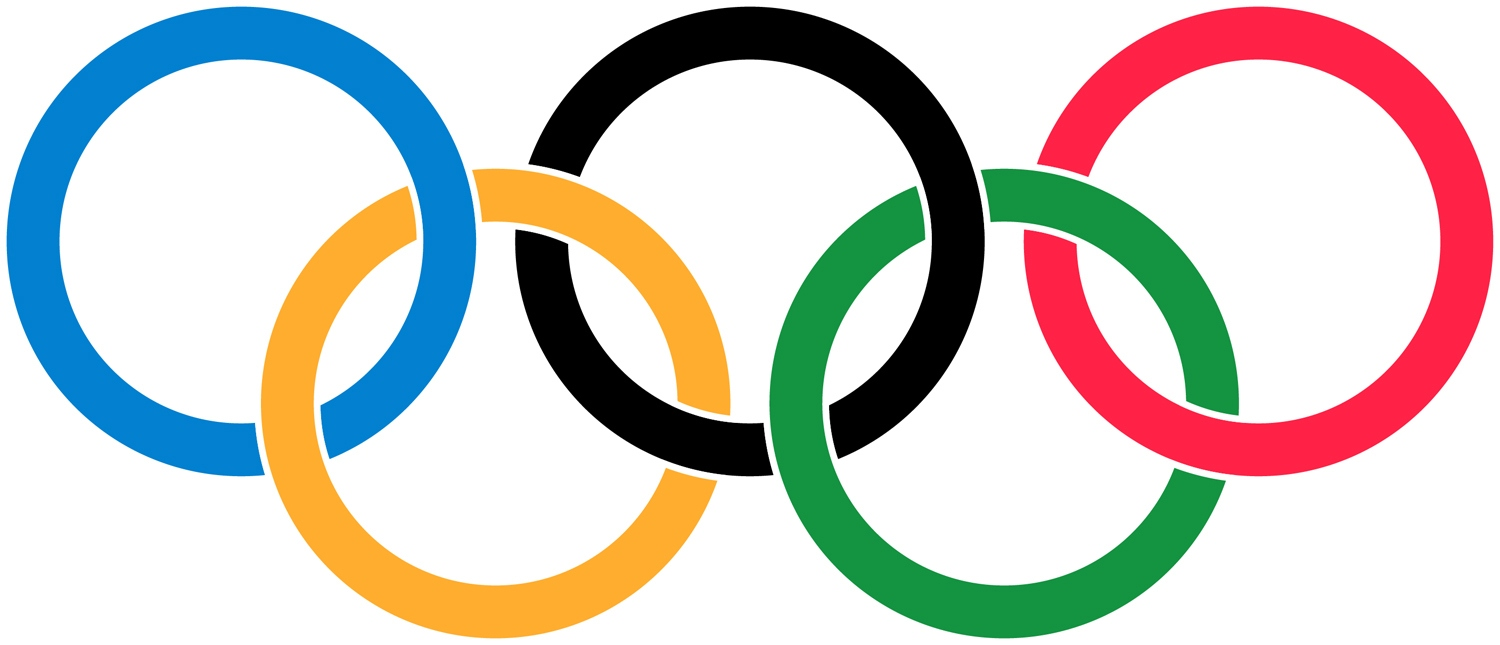
\includegraphics[width=0.55\textwidth]{images/circles/source/olympic.jpeg}
    \caption{Олимпийский флаг}
    \label{img:ol_logo}
\end{figure} 

Мы не имели никакого права не обратиться к произведениям основоположника абстракционизма и нашего соотечественника --- Василия Васильевича Кандинского:

\begin{figure}[ht!]
    \centering
    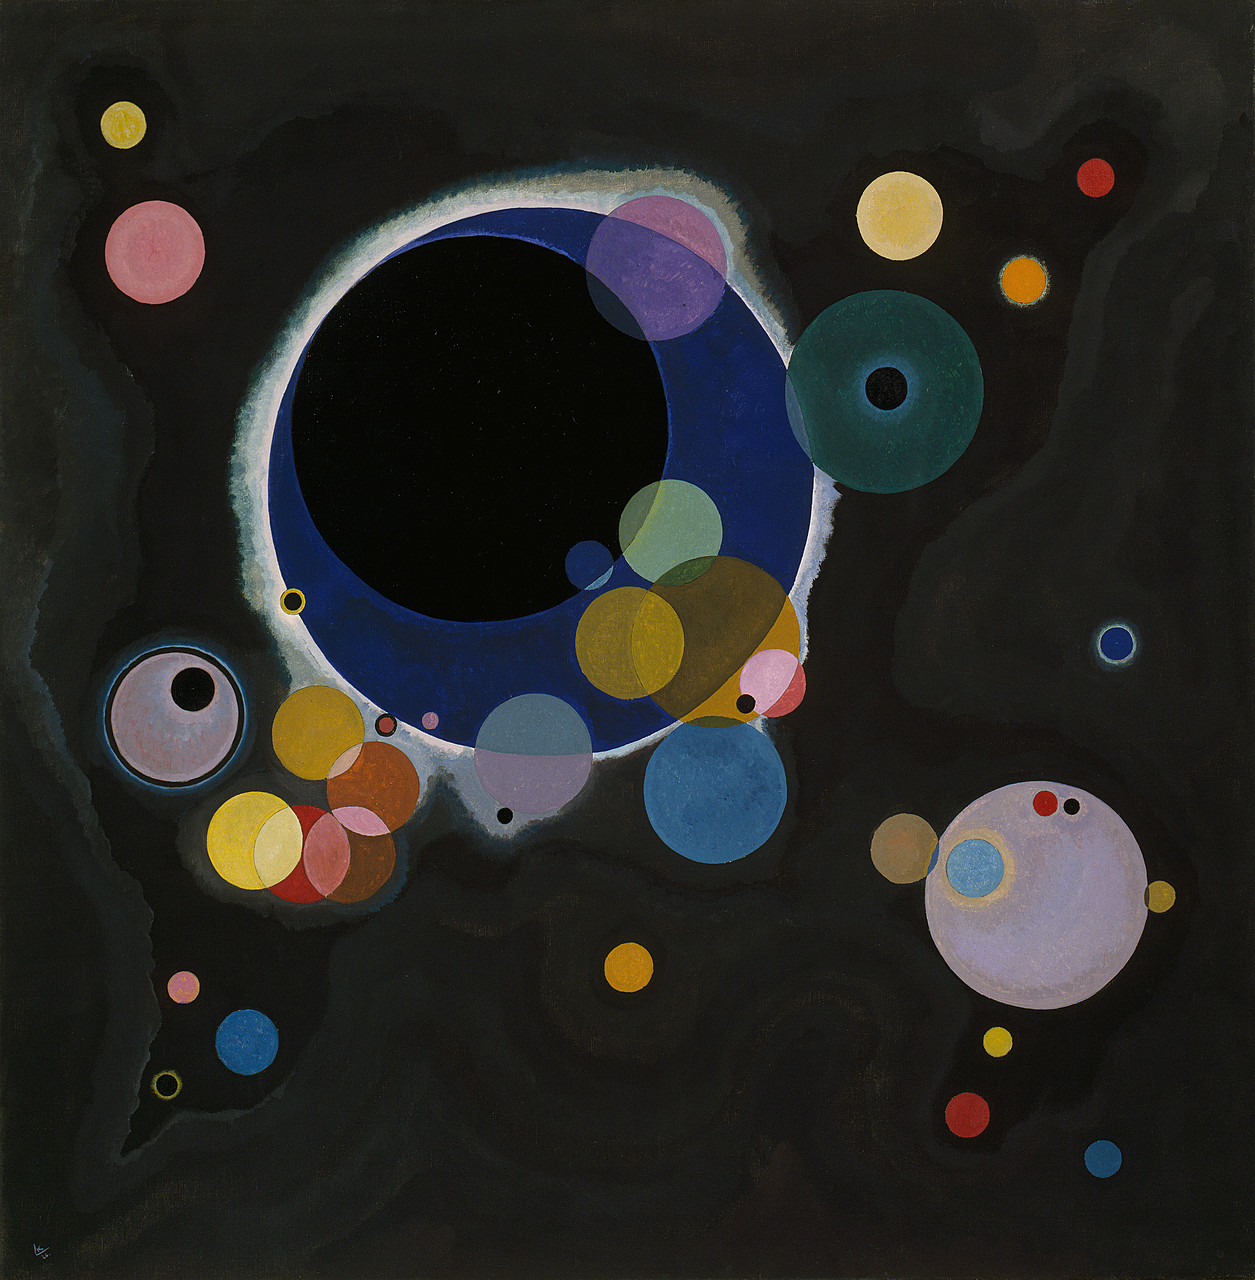
\includegraphics[width=0.55\textwidth]{images/circles/source/Kandinsky_Several_Circles.jpg}
    \caption{В.В. Кандинский -- Несколько кругов}
    \label{img:kan_logo}
\end{figure} 

\clearpage

Последним изображением стала фотография Mercedes-Benz 300 SEL AMG <<Красная свинья>>, ставший ключевым элементом в первом для новой компании AMG триумфе в автогонках:
\begin{figure}[ht!]
    \centering
    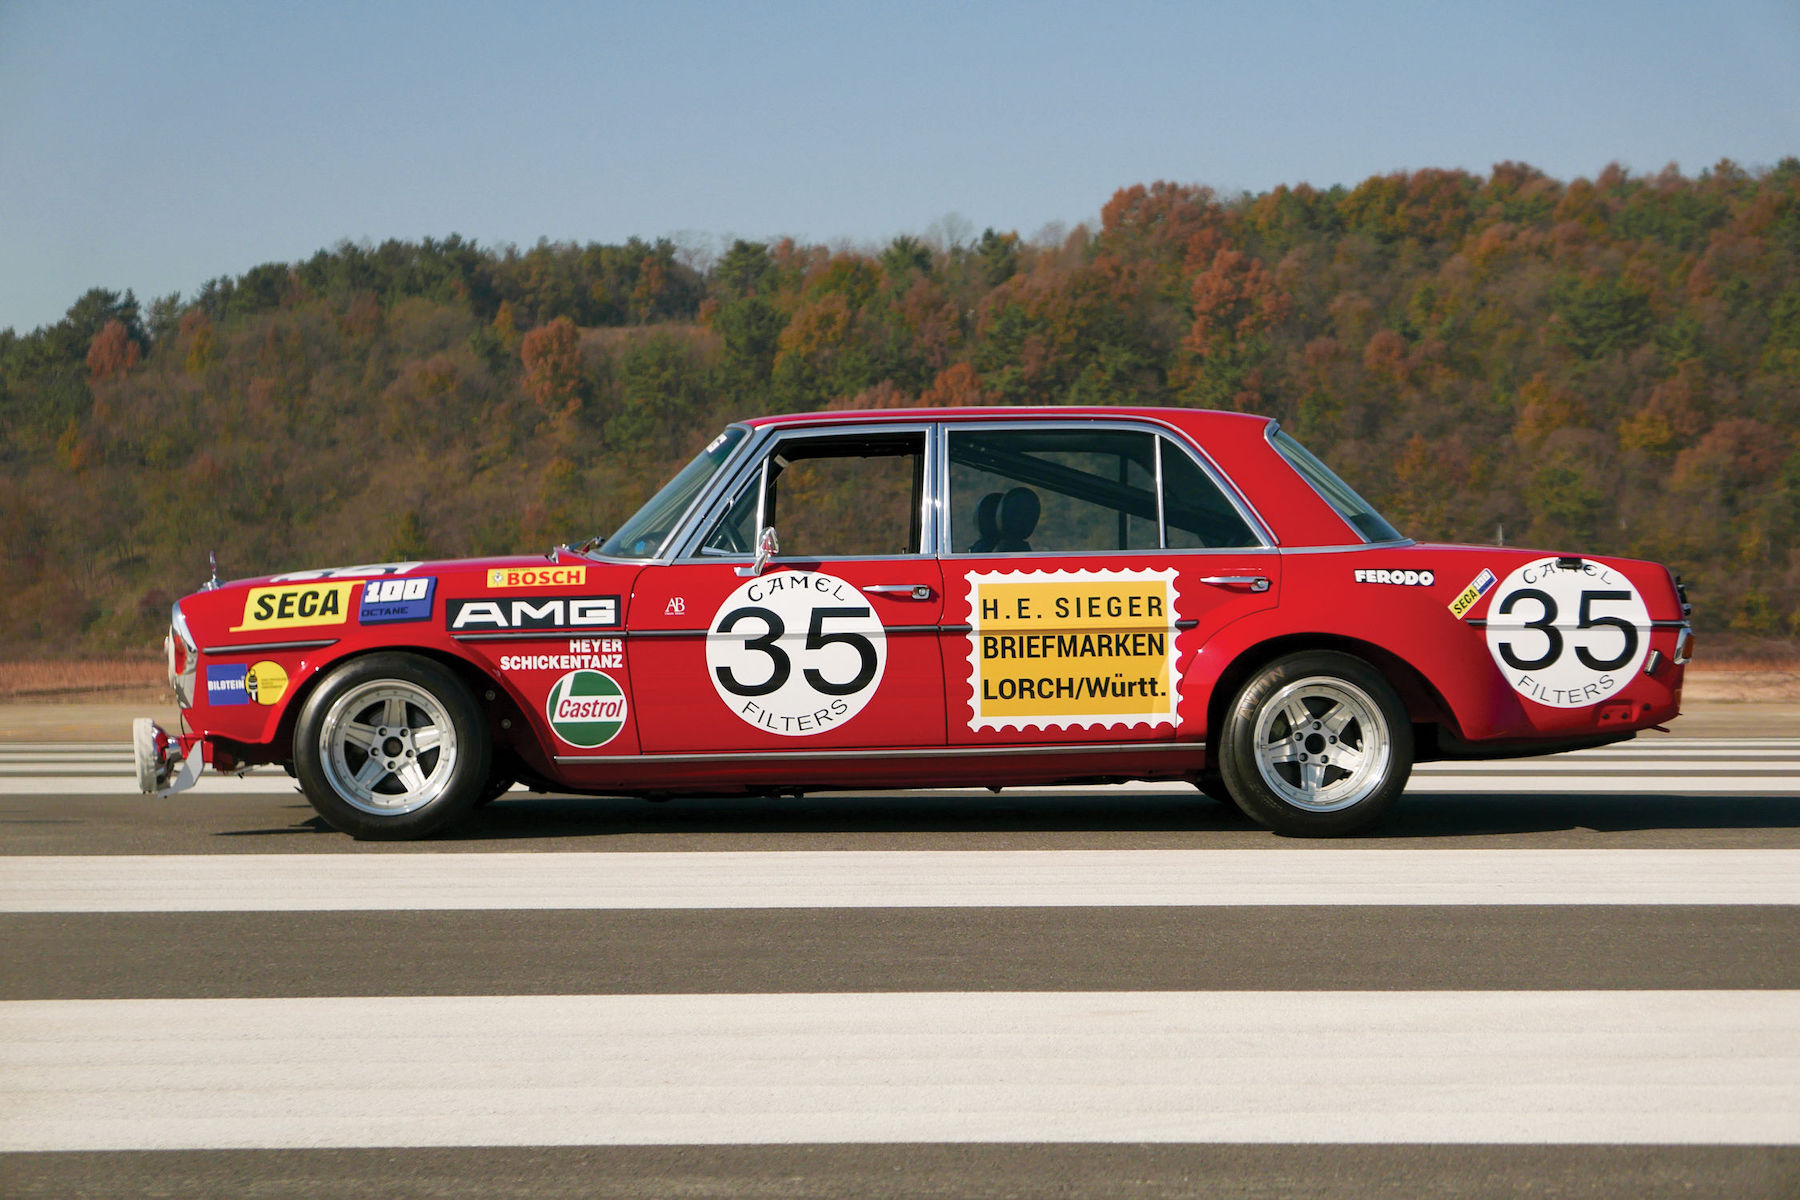
\includegraphics[width=0.55\textwidth]{images/circles/source/Mercedes 300 SEL 6.8 AMG red pig.jpg}
    \caption{ Mercedes-Benz 300 SEL AMG <<Красная свинья>>}
    \label{img:mr_logo}
\end{figure} 

\subsection{Программа на языке Python}
\begin{lstlisting}[caption={Исходный код функции для нахождения и отображения окружностей с помощью преобразования Хафа}, label={lst:line_compute}]
    def circle_detection(option, image):
        # creating image copies
        result = image.copy()
        result_r = image.copy()
        edged = image
        match option:
            case 0:
                # output of the original image
                cv.imshow('Source Image', image)
                cv.waitKey(0)
            case 1:
                # Hough transform
                # Specified radius
                hough_radius = np.arange(180, 181)
                # Getting Hough accumulator
                hough_res = skimage.transform.hough_circle(edged, hough_radius)
                # Getting coordinates for centers of circles 
                ha, cx, cy, radii = skimage.transform.hough_circle_peaks(hough_res, hough_radius, total_num_peaks=1)
                for center_y, center_x, radius in zip(cy, cx, radii):
                    # overlaying circles of specified radius
                    cv.circle(result, (center_x, center_y), int(radius), (255, 255, 0), 10, cv.LINE_AA)
                # Radius range
                hough_radius_r = np.arange(175, 239)
                # Getting Hough accumulator
                hough_res_r = skimage.transform.hough_circle(edged, hough_radius_r)
                # Getting coordinates for centers of circles 
                ha, cx, cy, radii = skimage.transform.hough_circle_peaks(hough_res_r, hough_radius_r, total_num_peaks=4)
                for center_y, center_x, radius in zip(cy, cx, radii):
                    # overlaying circles
                    cv.circle(result_r, (center_x, center_y), int(radius), (255, 255, 0), 10, cv.LINE_AA)
                # transferring recieved images and data to function of creating a comparative image
                image_displaying(image, edged, result, result_r, hough_radius[0], hough_radius_r[0], hough_radius_r[-1])
                # cv.imwrite('results/circles/Mercedes_SP.jpg', result)
                # cv.imwrite('results/circles/Mercedes_R.jpg', result_r)
            case _:
                print('Wrong option! Enter the right number')
    \end{lstlisting}

    \begin{lstlisting}[caption={Исходный код функции для создания сравнительного изображения с результатами преобразования}, label={lst:show_images}]
        def image_displaying(source, canny, finale, finale_r, sp, mn, mx):
            # creating figure with mosaic layout
            fig, axs = plt.subplot_mosaic([['src', 'can'], ['fin', 'finr'], ['info', 'infor']], layout='tight',
                                        figsize=(9.2, 7.8))
            # plotting images
            axs['src'].imshow(cv.cvtColor(source, cv.COLOR_BGR2RGB))
            axs['can'].imshow(canny, cmap=matplotlib.cm.gray)
            axs['fin'].imshow(cv.cvtColor(finale, cv.COLOR_BGR2RGB))
            axs['finr'].imshow(cv.cvtColor(finale_r, cv.COLOR_BGR2RGB))
            # turning off axes
            axs['src'].axis('off')
            axs['can'].axis('off')
            axs['fin'].axis('off')
            axs['finr'].axis('off')
            axs['info'].axis('off')
            axs['infor'].axis('off')
            axs['src'].set_title('Image')
            axs['can'].set_title('Canny edges')
            axs['fin'].set_title('Hough (Specified radius)')
            axs['finr'].set_title(' Hough (Range)')
            # plotting the specified radius size
            axs['info'].text(0.5, 0.5, f'Radius length:{sp}', size=25,
                            ha='center',
                            va='center',
                            bbox=dict(boxstyle="square",
                                    ec=(1., 0.5, 0.5),
                                    fc=(1., 0.8, 0.8)
                                    )
                            )
            # plotting minimum and maximum radius sizes
            axs['infor'].text(0.5, 0.5, f'Min radius: {mn}\nMax line: {mx}', size=25,
                            ha='center',
                            va='center',
                            bbox=dict(boxstyle="square",
                                        ec=(1., 0.5, 0.5),
                                        fc=(1., 0.8, 0.8)
                                        )
                            )
            # displaying and saving the plot
            plt.show()
            fig.savefig('results/circles/olympic.jpg')
            plt.close()
        \end{lstlisting}

\subsection{Результаты преобразования}

\begin{figure}[ht!]
    \centering
    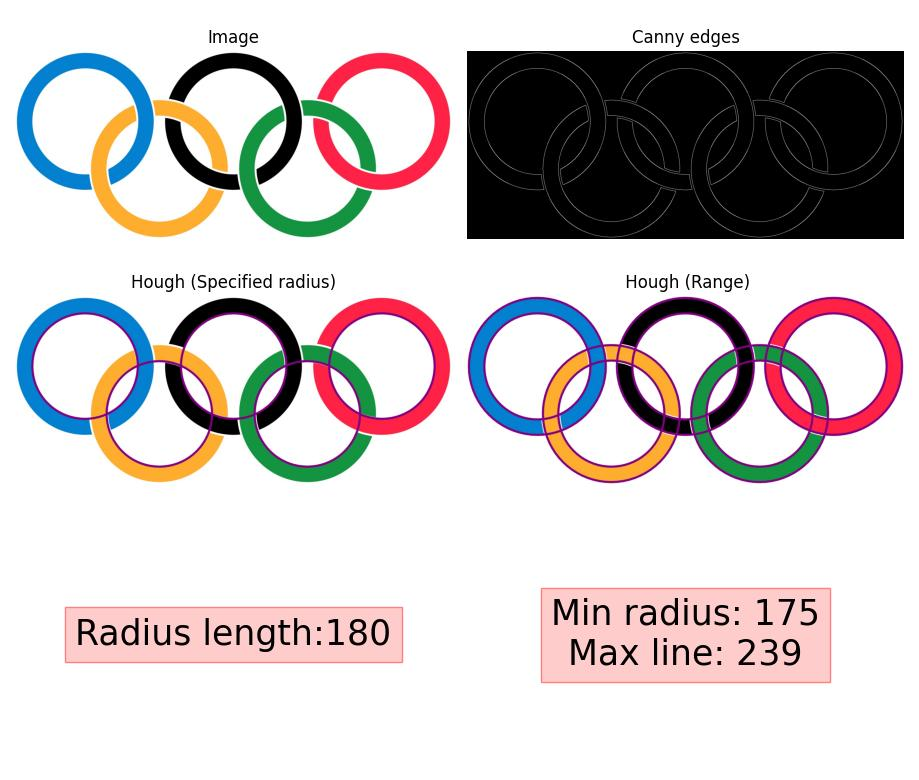
\includegraphics[width=0.8\textwidth]{images/circles/olympics.jpg}
    \caption{Исходное изображение 1; контуры изображения, полученные алгоритмом Кэнни; результаты преобразования Хафа для определенного радиуса и диапазона радиусов}
    \label{img:fin_ol}
\end{figure}

\begin{figure}[ht!]
    \centering
    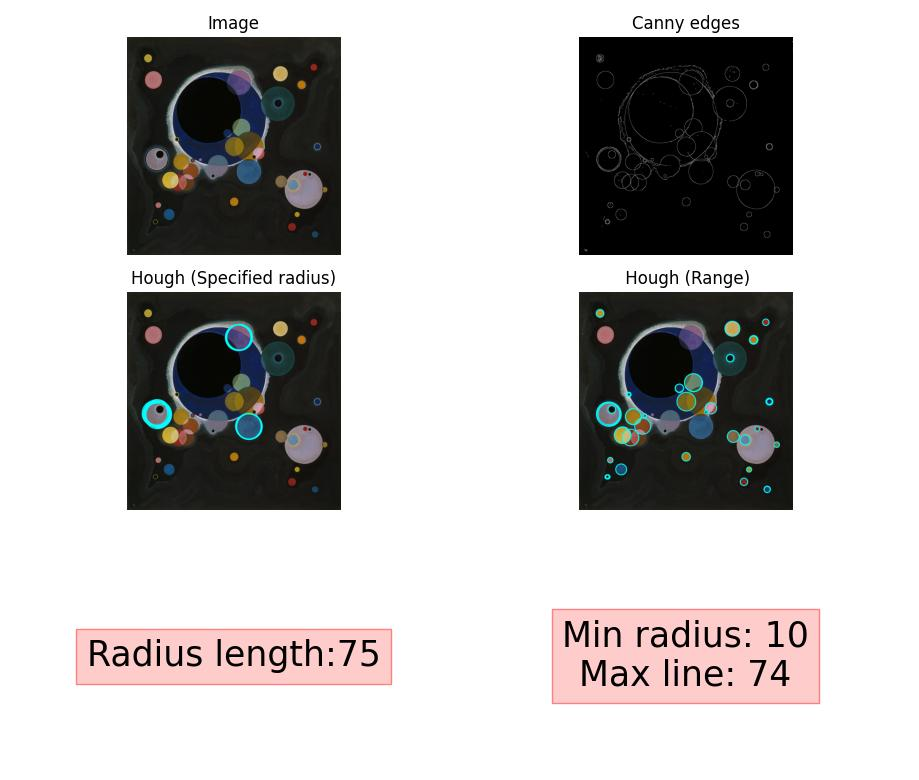
\includegraphics[width=0.8\textwidth]{images/circles/Kandinsky_Several_Circles.jpg}
    \caption{Исходное изображение 2; контуры изображения, полученные алгоритмом Кэнни; результаты преобразования Хафа для определенного радиуса и диапазона радиусов}
    \label{img:kan_fin}
\end{figure}

\begin{figure}
    \centering
    \begin{subfigure}[b]{0.4\textwidth}
        \centering
        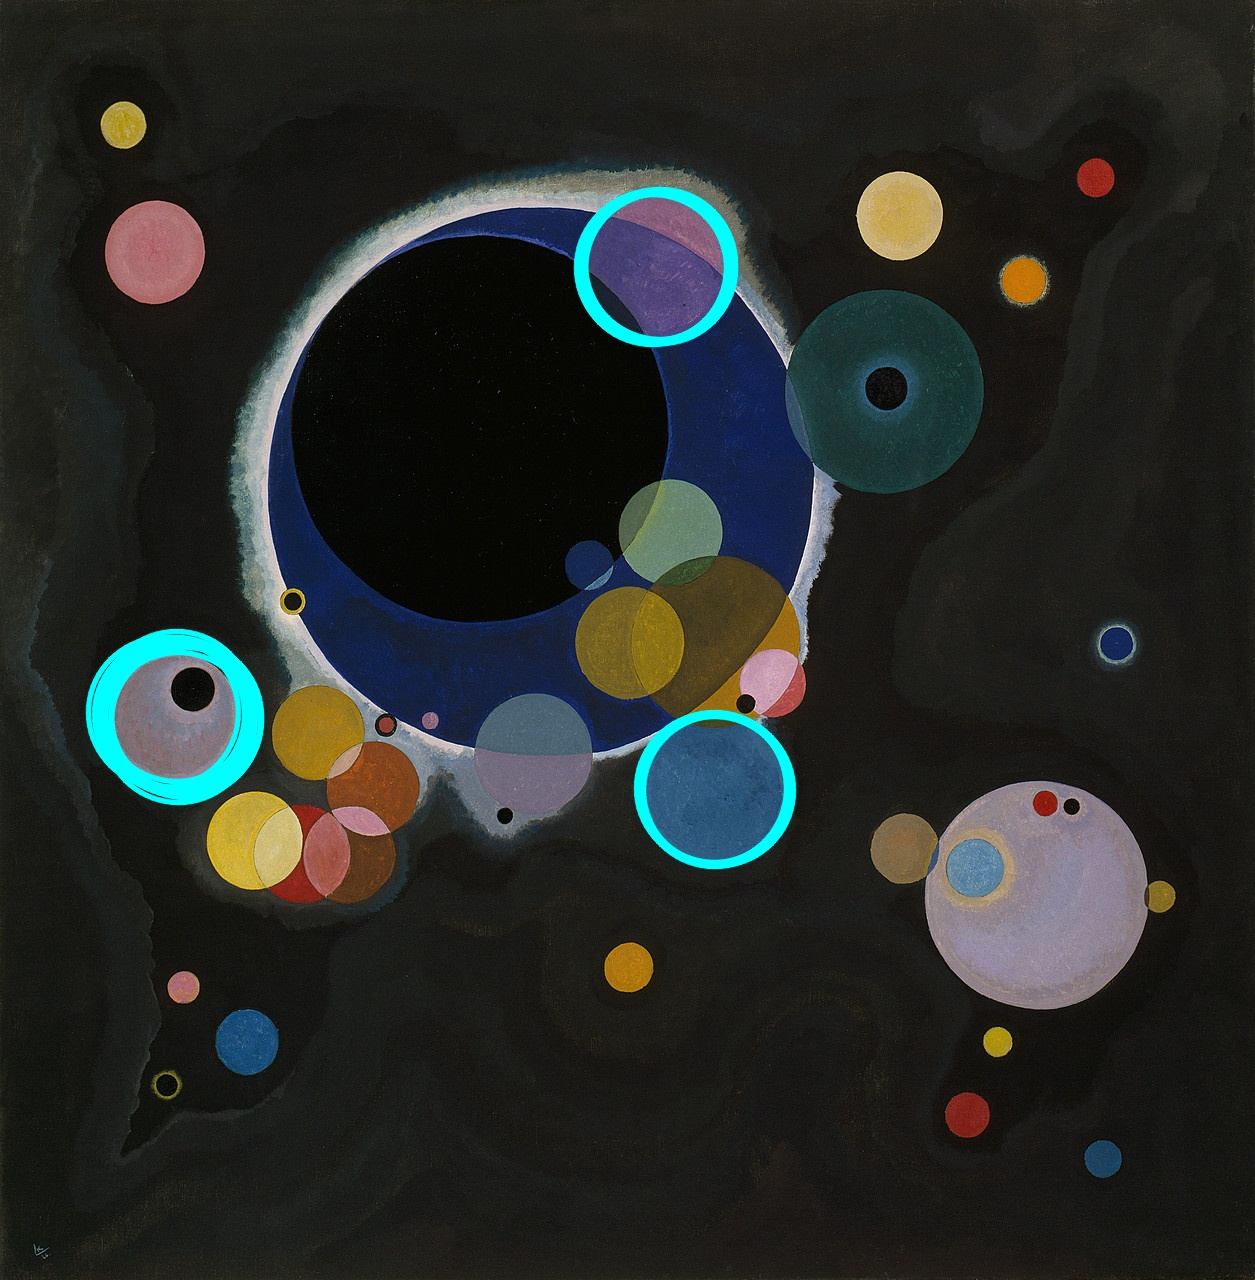
\includegraphics[width=\textwidth]{images/circles/Kandinsky_Several_Circles_SP.jpg}
        \caption{Результат преобразования Хафа для определенного радиуса окружностей}
        \label{img:kan_sp}
    \end{subfigure}
    \hfill
    \begin{subfigure}[b]{0.4\textwidth}
        \centering
        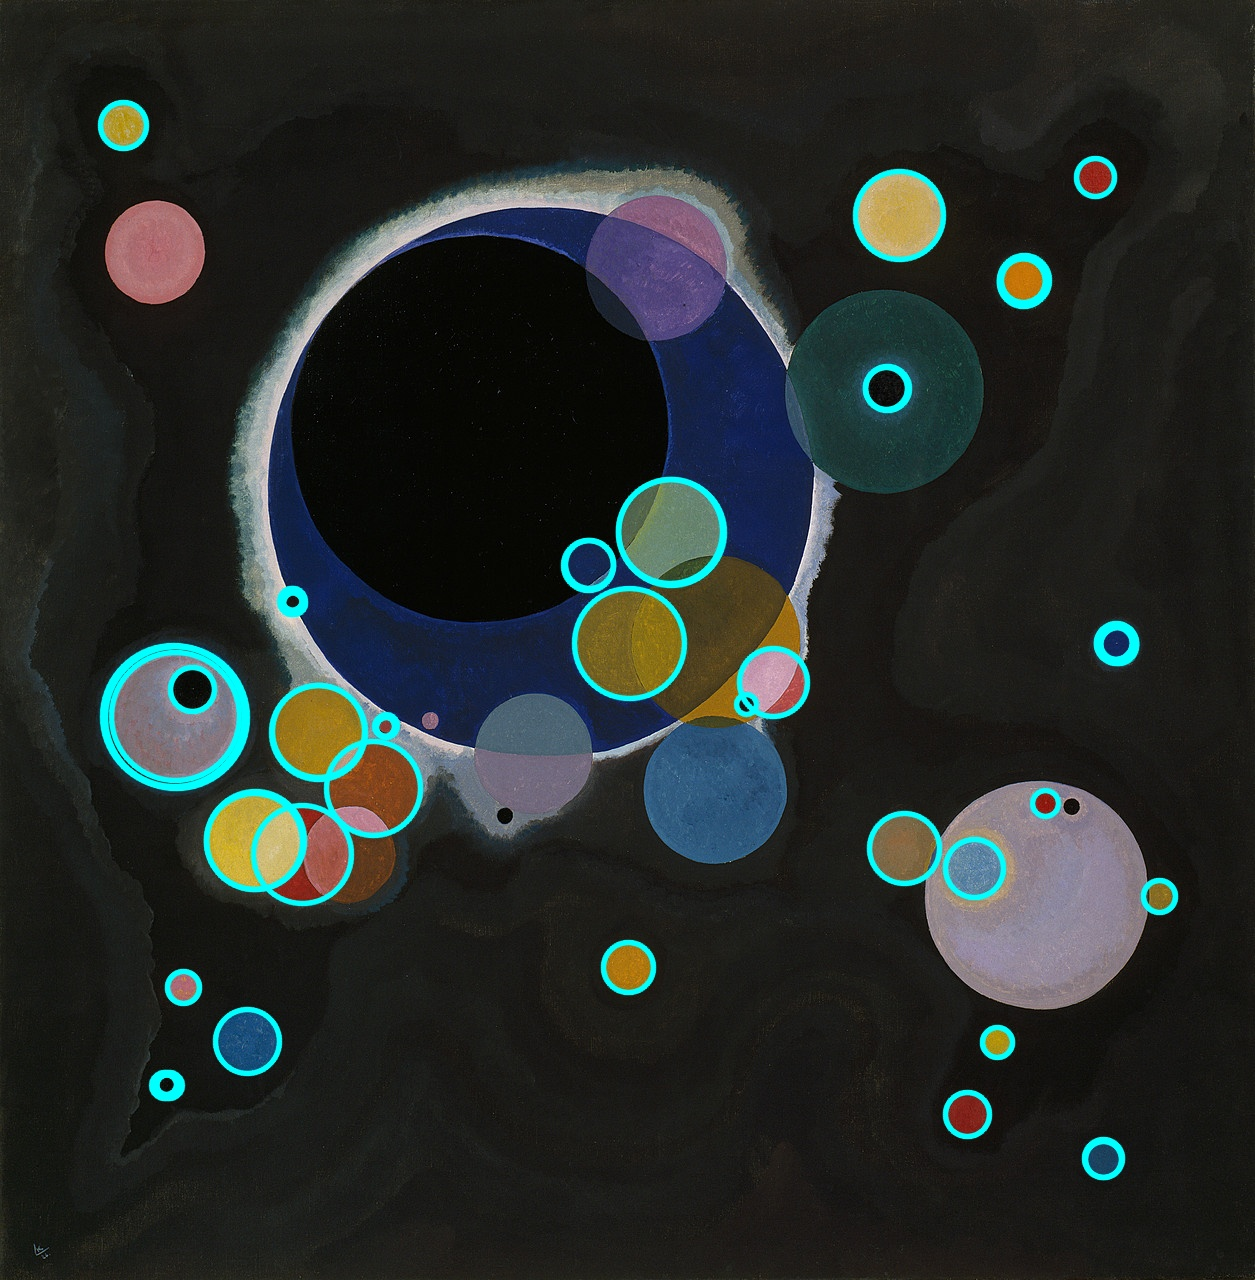
\includegraphics[width=\textwidth]{images/circles/Kandinsky_Several_Circles_R.jpg}
        \caption{Результат преобразования Хафа для диапазона радиусов}
        \label{img:kan_r}
    \end{subfigure}
        \caption{Результаты преобразования Хафа}
       \label{img::kan_comp}
\end{figure}

\begin{figure}[ht!]
    \centering
    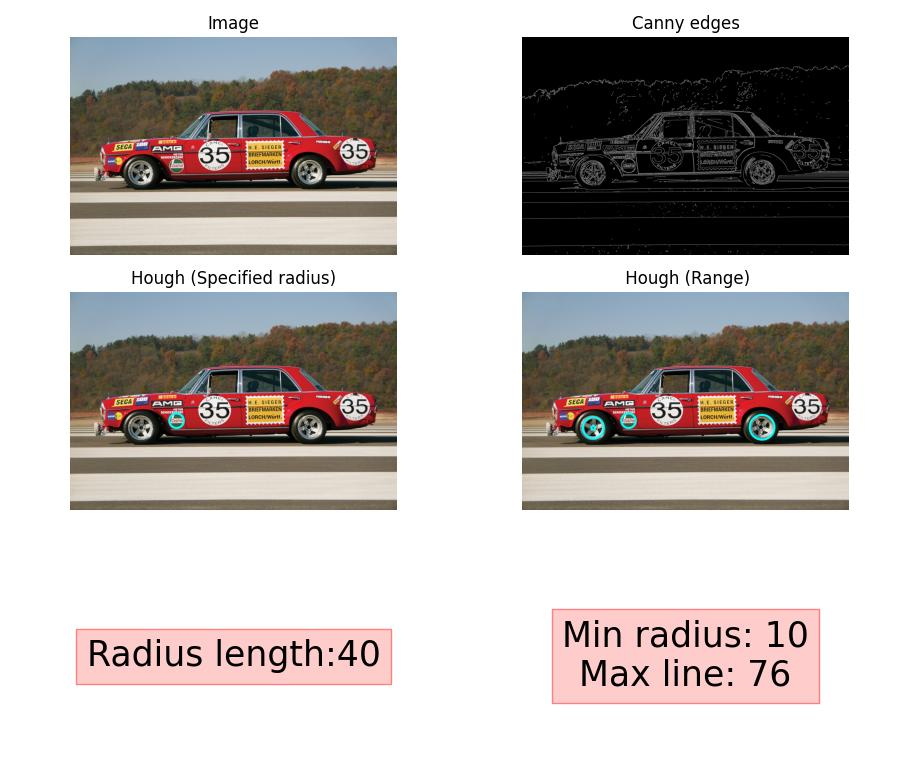
\includegraphics[width=\textwidth]{images/circles/Mercedes.jpg}
    \caption{Исходное изображение 3; контуры изображения, полученные алгоритмом Кэнни; результаты преобразования Хафа для определенного радиуса и диапазона радиусов}
    \label{img:mr_fin}
\end{figure}

\begin{figure}
    \centering
    \begin{subfigure}[b]{\textwidth}
        \centering
        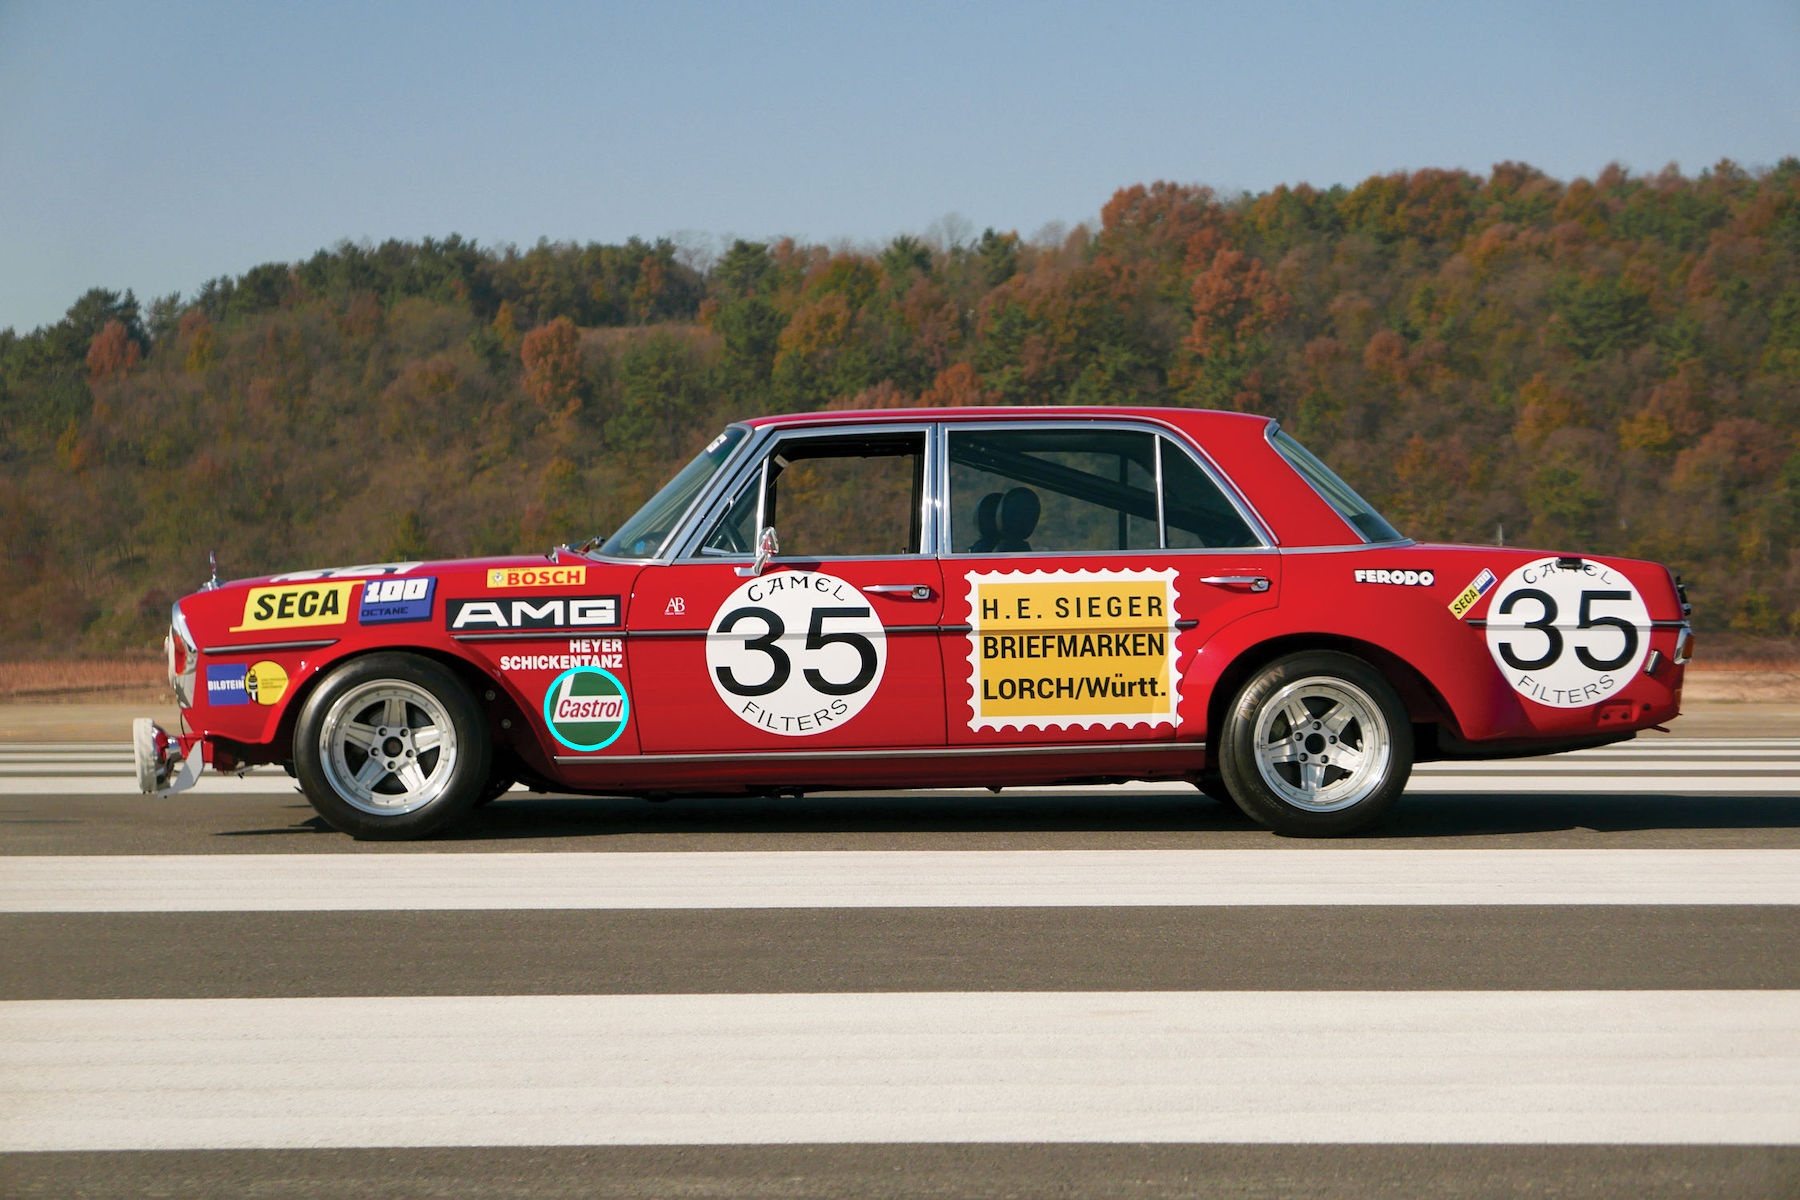
\includegraphics[width=\textwidth]{images/circles/Mercedes_SP.jpg}
        \caption{Результат преобразования Хафа для определенного радиуса окружностей}
        \label{img:mer_sp}
    \end{subfigure}
    \hfill
    \begin{subfigure}[b]{\textwidth}
        \centering
        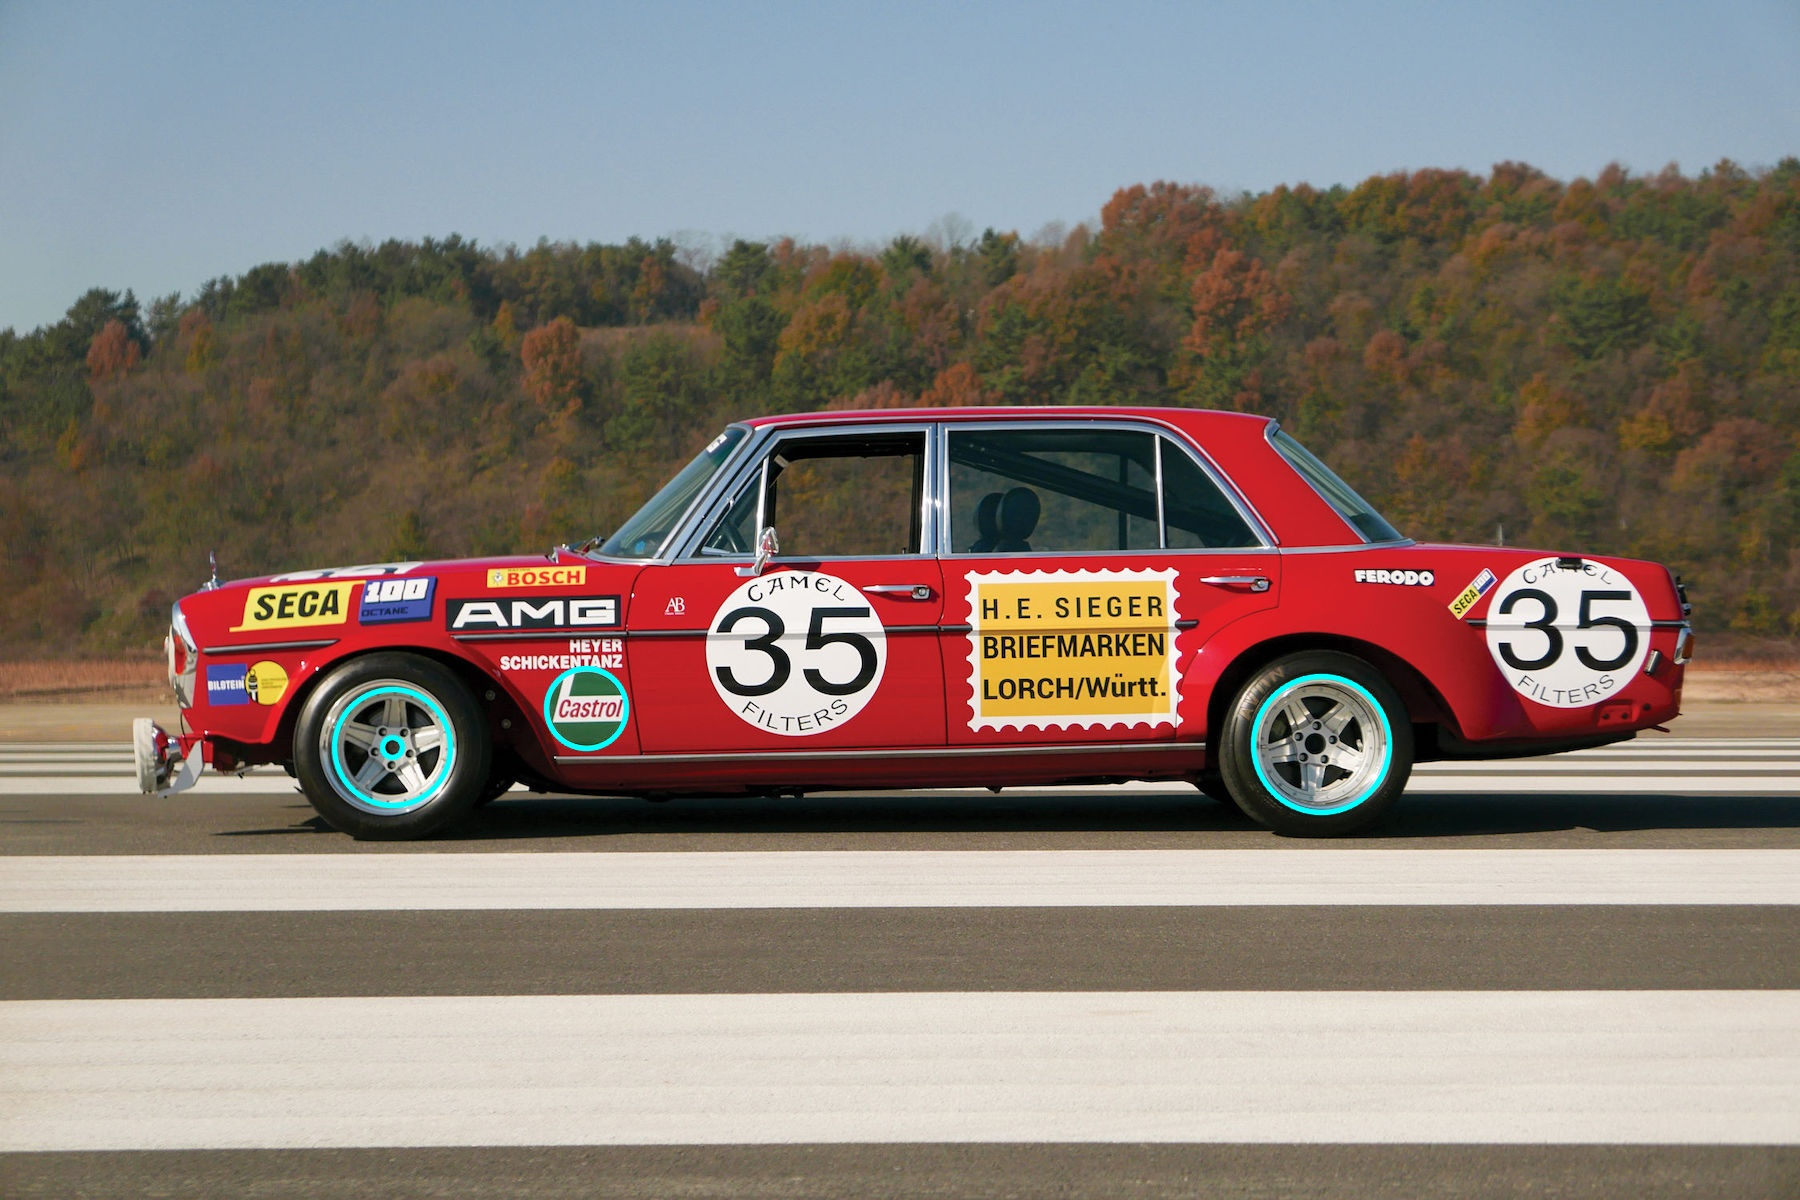
\includegraphics[width=\textwidth]{images/circles/Mercedes_R.jpg}
        \caption{Результат преобразования Хафа для диапазона радиусов}
        \label{img:mer_r}
    \end{subfigure}
        \caption{Результаты преобразования Хафа}
       \label{img::mer_comp}
\end{figure}

\clearpage